\section {Introduction}% (and Inspiration/Motivation)}
%\textbf{}
In this study, antonym pairings that were accepted before this work are refered to as \textit{institutional} or \textit{traditional} while those that were not are referred to as being \textit{non-institutional} or \textit{non-traditional}. Here, the behavior of nominal antonymy will be proven to differ from that of adjectival antonymy.  

%Since nouns such as $male$ \opp $female$, $feminine$ \opp $masculine$, $boy$ \opp $girl$ are generally accepted to be pairs of opposites, the term non-modified noun will be used to refer to non-gender nouns or nouns that are not modified by an adjective (e.g. red carpet).  Meanwhile, the term noun will be used in the general sense to refer to any noun, including abstract nouns.  The tilde, \oppnospace, will be used to denote an antonym pairing such as $hot$ \opp $cold$.  

In order to understand the full import of findings on nominal antonym, various observations will now be provided concerning \textit{abstract antonymy}. 

Although mathematical terms are used where possible, understanding them is not necessary for understanding the study.  They are meant to be observational and future work will be required to determine whether the same concepts apply to nominal antonymy.

In sections \ref{results}, \ref{conclusion} (Results, Conclusion), the following hypothesis will be proven:
	\begin{quote}
		$H_{1}:$ The mean number of antonyms that exist for a noun are greater is greater than the mean number of antonyms for an adjective.
	\end{quote}

%Sections~\ref{usages}-\ref{middle-ground} lend themselves to being described in mathematical terms while sections~\ref{usages}-\ref{middle-ground} do not.

%will follow concerning the possibility that abstracted application of the rules that govern institutionalized opposites is what govern the majority (if not all) of antonyms for unmodified nouns.  In other words, this study takes the step to determine whether rules for generation of standard antonyms can be applied more generally to even the most concrete of nouns, rules which must act in tak-like manner in order to apply more generally than they normally would.

\subsection {Selected Antonym Usages: Paradox and Middle-Ground} 
\label{usages}
Two usages of antonyms will be touched on here, \textit{paradox} and \textit{middle-ground}. For a discussion on other usages such as implicit and explicit comparison, \citeA<see>{Zhang}.  

Antonyms can be used together to create two phenomena: (1) a paradox, and (2) a middle-state or middle-ground.  It is up to natives of a language to determine which usage is created by a given pair.  Gradability probably plays a role in this.  This will be explored in section~\ref{classification}.

\subsubsection{Paradox}
Citing a Latin example \textit{neque vivus neque mortuus} (not alive not dead), Bertocchi notes that antonyms can be used to create a paradox (Bertocchi 2003).  

\subsubsection{Middle-Ground}
The same construction that can be considered paradoxical can also be used to suggest a middle-ground.  Take for example the case of $hot$ \opp $cold$, forming the phrase \textit{not hot not cold}.  This is simply another way to express the middle-ground, \textit{warm}.  Interestingly, a word for the middle-state need not exist to detain the pair from creating a paradox.  Take the pair $tall$ \opp $short$.  One might say that the obvious between-state is \textit{medium}.  However, that does not always work for although one can say ``I am tall/short'', one cannot simply say ``I am medium'' without the accompaniment of the word \textit{height}.  Whether this is an exception or phenomenon in English is left to future work.  Nevertheless, the fact stands that in English an exact word for the middle-state need not exist seems to hint that a given antonym pair can create either a paradox or a middle-ground and it is up to the native to determine which it is.  

%In some given language a term for medium may not exist and whether it is paradoxical or not is up to the native speakers of the language.  Meanwhile, languages which have a form to describe medium would say it is simply a middle ground and not a paradox. 

%\subsubsection{Discussion: Creating Middle-Ground for Nouns}
%Preliminary work showed that antonyms for nouns exist (not published; xyz).  Let's try to create a middle-ground for $pencil$ \opp $pen$.  Using the aforementioned syntax construction, we would end up with \textit{neither pencil nor pen}.  Indeed, this seems to work superficially, but one might ask whether one could use a paraphrase to describe what is really meant (is it an erasable pen or a permanent pencil?).  
%The speaker does not choose to select something which would fit the criteria, perhaps because they do not know that erasable pens exist.  The speaker uses opposition, two extremes, to create an enclosure automatically defining the possible characteristics (or non-characteristics) that are inherent in the desire.  In this case, the speaker highlights key characteristics by saying ``something that looks like a pen, but that is still erasable.''

\subsection {Classification: Gradable vs. Non-gradable}
\label{classification}
Two main types of antonyms exist: gradable and non-gradable. Bertocchi calls gradable antonyms \textit{contraries}, while non-gradable antonyms are \textit{contradictories}.   Non-gradables, or contradictories are binary, but also have no middle ground (Bertocchi 2003).  By this criterion, $alive$ \opp $dead$ constitute a contradictory while $tall$ \opp $short$ do not.  In other words, if there is a continuum between the two (non-binary), then it is gradable an a paradox will not be formed. 

In mathematical terms: 
	\begin{quote}
		The set of \textit{gradables}, $G$, is defined $s.t.~ \forall x \in G~\exists y~s.t. (x+y)/2$ exists.

		The set of \textit{non-gradables}, $G$, is defined $s.t.~ \forall x \in G~\exists y~s.t.~x\not=y$, $(x+y)/2$ does not exist.
	\end{quote}

%This study will reveal the existence of a greater number of categories for concrete antonyms than for abstract nouns. 

\subsection {Attributes of Traditional Antonymy} 
Besides the ability to be classified as either gradable or non-gradable, antonyms tend to binary, communicative, and transitive. These will now be defined and discussed, with examples.  

\subsubsection {Dichotomy} 
Traditional opposites tend to be binary or dichotomous.  Lindner states ``The opposition relation is built squarely on a dichotomy or binary contrast of some sort.'' (Lindner 1982) In such cases, one term can be understood by using the negated form of its opposite.  This works only when considering optimal pairing partners for a given adjective.  Take for example \textit{small}.  Both \textit{big} and \textit{large} could be accepted as opposites, but depending on the circumstance, \textit{big} or \textit{large} is the optimal partner.

In mathematical terms: 
	\begin{quote}
		The set of \textit{gradables}, $G$, is defined $s.t.~G \in \mathbb{R}~and~\forall x \in G~\exists y \in G~s.t.~x\not=y$, $(x+y)/2$ exists.

		The set of \textit{non-gradables}, $G$, is defined $s.t.~G \not\in \mathbb{R}$ and $s.t.$ $m$, the arithmetic mean of two elements $a, b \in G, \not\in G$.
	\end{quote}

\subsubsection {Communicativity} 
To be communicative, given one adjective $X$ whose best opposite is $Y$, $Y$’s best opposite must be $X$.  This is easily the case for traditional antonyms as they tend to be contained in obviously binary sets. In mathematical notation, where  denotes two-way implication.  In mathematical terms this would be: 
	\begin{quote}
		$(X$ \opp $Y) \Leftrightarrow (Y$ \opp $X)$
	\end{quote}

\subsubsection {Transitivity} 
For adjectives (and abstract nouns), one can find the antonym for word $X$ by finding an antonym, $Y$, for one of $X$’s synonyms, $Z$.  This is a transitive process.  In a mathematical notation where ``='' denotes synonymy, this would be: 
	\begin{quote}
		$X = Z, (Z$ \opp $Y) \Leftrightarrow (X$ \opp $Y)$
	\end{quote}

\subsection {Discussion: Institutional Paradox}
\label{paradox} 
In English, there are words for which antonyms are well-known or institutionalized.  These include adjectives, adverbs, and some abstract nouns (depending on the dictionary).  In other words, for a given instance of an abstract part of speech, say an adjective, there exist a corresponding synonym(s) and antonym(s).  However, for concrete parts of speech like a noun, only synonyms seem to be institutional. This presents an institutional paradox in which abstract terms can undergo a process or rule to generate an opposite, but the underlying rule that functions so easily upon abstract parts of speech does not work as prevalently on more concrete parts of speech!  Figure ~\ref{fig:introFig} visualizes this paradox.

Gender nouns and modified nouns (nouns whose connotation carries the connotation describable by an adjective) are marked in red in Figure ~\ref{fig:introFig} because they act differently than normal nouns; they have corresponding antonyms in spite of the fact that they are concrete.  For adjectivally-modified nouns this is also the case, probably due to the presence of the adjective for which antonymy is institutional.  Gender nouns act as if they are adjectivally-modified nouns, perhaps because they are modified internally (charged with adjectival meaning).  Since adjectives tend to be binary (when an opposite exists), the modified and gender nouns are polarized, meaning that they have an optimal pairing such that two extremes within a class are created.  Example pairs include: $female$ \opp $male$, $man$ \opp $woman$, $negative~electron$ \opp $positive~electron$, $hen$ \opp $tom$, $boy$ \opp $girl$.  Note that some of these nouns can be used as adjectives ($female$ \opp $male$, $novice$ \opp $expert$), and perhaps that is where their dichotomy was born.  Such pairings are binary---an attribute typically observed in adjectives as far as antonyms are concerned.  Gender nouns and modified nouns are indeed exceptional.  Whether they are more concrete than abstract is up for question.  Figure~\ref{fig:introFig} treats them as highly concrete.  Perhaps they are both.    

\begin{figure}[here]
	\centering
	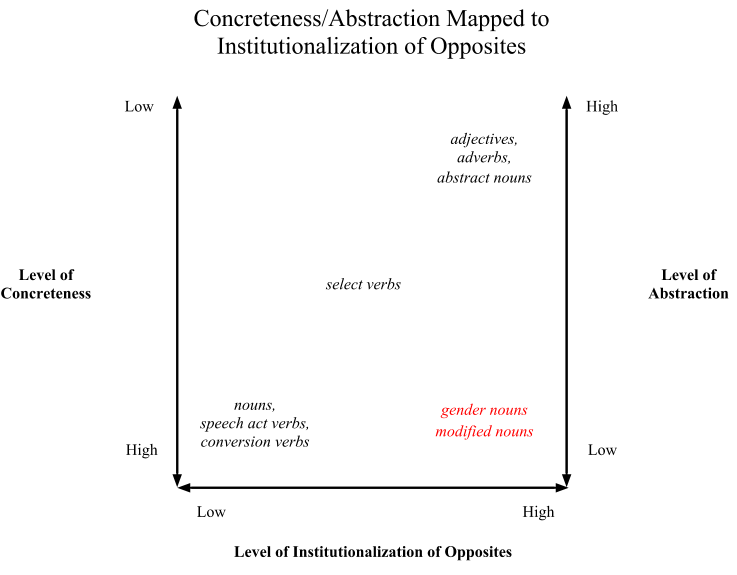
\includegraphics[width=0.9\textwidth]{images/Diagram.png}
	\caption{Concreteness/Abstraction mapped to institutionalization of opposites.  Red is used to demarcate word types which are marked.}
	\label{fig:introFig}
\end{figure}
	
Note also that abstract nouns are listed separately from adjectives and adverbs; although they are classified as nouns, they are abstract.  They are nouns because they can be treated as subjects in a sentence and can receive many of the same theta roles that concrete nouns receive.  
Antonyms for abstract nouns are institutionalized just as those for adjectives are.  Examples include: $belief$ \opp $disbelief$; $faith$ \opp $skepticism$; $love$ \opp $hatred$; $hope$ \opp $discouragement$, $hopelessness$; $unity$ \opp $disunity, partiality$.

%\subsubsection {Adjective vs. Nouns Vs. Adjectivally-Modified Nouns}
%Traditionally, adjectives can have both antonyms and synonyms, while non-modified nouns can have only synonyms.  This would make it difficult to define a concrete noun based on its opposite—unless it is modified.  Thus, to describe a house in terms of its opposite is traditionally impossible, unless it is described as being tall, in which case part of its definition could describe it as not short.  So, when concrete nouns are modified, a portion of their definition may include its antonym.  This is a contrived example, but one might imagine a more complex adjective modification that lends itself more towards definition via description in terms of opposites than by traditional means of definition.  

\subsubsection {Opposition in Semantic Primitives} 
Semantic primitives make up the core meaning of language (Wierzbicka 2009).  Wierzbicka says that semantic primitives are only definable in terms of themselves.  Interestingly, in her list of semantic primitives she includes a negating mechanism, NOT (Wierzbicka 2009).  It is this very mechanism which leads one to believe that opposition exists at the root of the meaning of language.  However, it remains to be proven how various parts of speech behave in the atmosphere of antonymy.  This is why proving the hypothesis $H_{1}$ is important.

%

\subsection {Side A.} Wilbur in his book “Opposites” mentions for various words.  Interestingly, after each keyword and opposite, he often decides to list another opposite (Wilbur 1921).  He often does this comically by playing off ambiguities such as word senses (e.g. bat as an animal or as a sporting instrument).  Occasionally, on a more serious note, he lists multiple opposites for words which are not ambiguous, such as earth.  Wilbur accepts the possibility of opposites for non-modified nouns and in some cases agrees with the possibility of more than 1 opposite.  His opposite for earth is sky or heaven; squash, bean; hat, shoes; present, past or future.

Lindner works to diffuse the confusion surrounding directional opposites.  She says “The opposition relation is built squarely on a dichotomy or binary contrast of some sort.  That is, iron, gold, silver, etc., may make up a contrast set or multiple taxonomy, but typically only members of a binary taxonomy are called opposites.  Furthermore, the notion of opposition is based on contrast within similarity (Lyons 1977:286)—that is, there must be some reason to compare two lexical items, so that we would want to call man and woman opposites, but not rose and pig” (Lindner 1982). Lindner agrees that boy \opp girl (concrete nouns), female \oppmale (abstract nouns/adjectives) are acceptable binary contrast sets.  However, since words are being generated as language changes, perhaps this number of binary pairs should be fluctuate and change.  Lindner might accept laptop \opp desktop, Mac \opp PC, or mountain \opp valley. 

In prototype theory, nouns can be grouped and classified.  Visually, they can be represented as being more or less distant from the core idea that they represent (Lakoff 1999).  For example, the word bird is a class of animals for which robins are good examples, but emus are not.  This theory might explain the existence of antonyms for non-modified nouns by arranging nouns in a multi-dimension arena, with various connection types connecting nouns to other nouns.  One connection type might link characteristics in common, while another connection type might denote dissimilarity.  Locating the best opposite for a given noun may be as simple as traversing connections or pathways in a certain way.  Perhaps one could traverse the pathways a given number of steps in certain directions; perhaps one could detect which words are mostly similar but somewhat different by using the using the number of like- and unlike -connections.  This would allow for the detection of contrast within similarity that Lindner mentioned.  

As mentioned in 1.3.1., Wierzbicka’s framework of semantic primitives contains the ability to negate.  Assuming the existence of semantic primitives, antonymy beyond the well-accepted antonymy for abstracts is not extreme.  Meaning itself depends on it.

\subsection {Side B.} Admittedly, Lindner seems to prefer that the term opposite maintain a strict traditional usage rather than a usage which can be applied to societally-determined antonyms for non-modified nouns.  Perhaps only gender nouns are acceptable to her.  It is difficult to tell since she only lists man \opp woman and *rose \opp pig.  

Thesauri or dictionaries that list synonyms and antonyms readily do so for adjectives and gender nouns, but not for non-modified nouns, except indirectly.  Some online dictionaries and synonym/antonym finders are described below.
	•	http://www.merriam-webster.com/thesaurus—does not list opposite for binary concrete nouns such as girl/boy, but does for female/male but does for adjectives such as hot/cold.
	•	http://dictionary.reference.com/—does not list opposite for binary girl/boy nor for female/male, but does for hot/cold.
	•	http://www.synonym.org/—does not list opposite for binary girl/boy nor for female/male, but does for hot/cold.

Only some dictionaries allow for girl/boy or female/male, although listings for adjectival antonyms hot/cold are acceptable.  This dearth of listings of concrete antonyms demonstrates that institution has not accepted the possibility of antonyms for non-modified nouns. 

The only other opposition against the possibility of antonyms for non-modified nouns is the overwhelming amount of studies performed for traditionally institutionalized sets of opposites and lack of studies on antonyms for non-modified nouns.  
